\documentclass[a4paper,12pt,oneside,openright]{report}% HEAD SECTION ->

\usepackage		 {a4wide  }% Don't waste place on the page.
\usepackage[T1]    {fontenc }% Allow accented output charachters
\usepackage[utf8]  {inputenc}% Allow accented input charachters 
\usepackage        {lmodern }% Modern output font	
\def\magyarOptions{suggestions=no}
\usepackage[magyar]{babel}	   % Set document language to use
\usepackage		 {amsmath}%Math mode additions
\usepackage		 {floatrow}% Append additional information to images (source)

\usepackage[pdftex]{graphicx}% Adds the ability to include images 
\usepackage        {color   }% Colors are fun :)
\usepackage        {colortbl}% Named even more. 
\usepackage        {url     }% Makes urls clickable 
\usepackage		 {minted  }% Code syntax highlighting 

\usepackage		 {tikz	  }% Latex drawn figures
\usetikzlibrary	 {matrix  }
\usepackage        {scalefnt }% Scale the latex drawn figure elements

% The csquotes should be used with bable to help with the references formating 
\usepackage[style=english]{csquotes} 
% Biblatex
\usepackage[style=ieee,
backend=biber,babel=other*, language=english, sorting=none,
backref=false]{biblatex} \DeclareSourcemap{ % Unfortunetly the
% bibtex currently knows of online type, not webpage. For now just map it.
  \maps[datatype=bibtex]{
    \map{
      \step[typesource=webpage, typetarget=online]
    }
  }
}

\addbibresource{./bibliography/main.bib}
% Smiley commands
\newcommand{\smiley}{\tikz[baseline=-0.75ex,green]{
    \draw circle (2mm);
\node[fill,circle,inner sep=0.5pt] (left eye) at (135:0.8mm) {};
\node[fill,circle,inner sep=0.5pt] (right eye) at (45:0.8mm) {}; \draw
(-145:0.9mm) arc (-120:-60:1.5mm);
    }
}

\newcommand{\frownie}{\tikz[baseline=-0.75ex,orange]{
    \draw circle (2mm);
\node[fill,circle,inner sep=0.5pt] (left eye) at (135:0.8mm) {};
\node[fill,circle,inner sep=0.5pt] (right eye) at (45:0.8mm) {}; \draw
(-145:0.9mm) arc (120:60:1.5mm);
    }
}

\newcommand{\neutranie}{\tikz[baseline=-0.75ex,black]{
    \draw circle (2mm);
\node[fill,circle,inner sep=0.5pt] (left eye) at (135:0.8mm) {};
\node[fill,circle,inner sep=0.5pt] (right eye) at (45:0.8mm) {}; \draw
(-135:0.9mm) -- (-45:0.9mm);
    }
}
% Background highlight color used for the source code and the tables
\definecolor{bgSrc}{rgb}{0.95,0.95,0.95}

\usepackage		   {hyperref}% - Add links between the doc
\usepackage[all]{hypcap}
\usepackage[numbered,
			  open, 
			  openlevel=2,
			  atend]{bookmark}% - We want numbers

\begin{document}

% A címlap
% !TeX encoding = UTF-8 
% !TeX spellcheck =hu_HU

\begin{titlepage}
\newcommand{\HRule}{\rule{\linewidth}{0.5mm}}
\begin{center}


\includegraphics[width=0.5\textwidth]{./kepek/Budapest-logo.jpg}\\
\textsc{Budapest Műszaki és Gazdaságtudományi Egyetem}\\
\textsc{Villamosmérnöki és Informatikai Kar}\\
\textsc{Adatbázisok Oktatási Labor}\\[1.5cm]
\textsc{Adatbázisok haladóknak -- VITMAV12}\\[0.5cm]

% Title
\HRule \\[0.4cm]
{ \huge \bfseries Oszlopcsaládok}\\[0.4cm]
{Cassandra és HBase}

\HRule \\[1.5cm]

% Author and supervisor
\begin{minipage}{0.4\textwidth}
\begin{flushleft} \large
\emph{Szerző:}\\
\textsc{Gábor} Bernát
\end{flushleft}
\end{minipage}
\begin{minipage}{0.4\textwidth}
\begin{flushright} \large
\emph{Vezető tanár:} \\
 Dr.~\textsc{Gajdos} Sándor
\end{flushright}
\end{minipage}

\vfill
% Bottom of the page
{\large \today}
\end{center}
\end{titlepage}

\tableofcontents

\listoffigures

\listoftables

\begin{abstract}
A Google a $2000$--es években azt tapasztalta, hogy nagy adat mennyiségek
hatékony eltárolására és feldolgozására a relációs adatbázisok már küszködnek.
Nem az adat mennyiség feltétlen a gond, hanem annak megbízható eltárolása és
gyors feldolgozása.

Ennek orvosolására megalkották a saját fájl (Google File System), adattároló
(BigTable) és adatfeldolgozó (MapReduce) rendszerüket. A problémával az Amazon
is hamarosan szembesült, és saját rendszerük megkötései és prioritásai szerint
létrehozták a Dynamo adat tároló rendszert.

E rendszerek közös és központi tulajdonságai az elosztottság (sok gép együtt,
mintsem kevés erős) és a magas redundancia szint biztosítása (adat nem veszhet
el). Ugyanakkor az adatokat főleg oszlopokba rendezve tároljuk el. Az ár, amit
fizettünk ezért, hogy a régi relációs adatbázis megközelítést, elvek egy részét
mögöttünk kell hagynunk, és új adattárolási paradigmákat kell megismernünk.

Az oszlop orientált adat tárolás koncepció nem újak. OLAP rendszerekben már több
évtizede jelen vannak relációs adatbázisokban. Az oszlop család megfogalmazást
főleg e rendszerekre illenek. Az iparba a MonetDB, Sysbase avagy Vertica
implementációi tűntek ki az évek során.

Az angol szakirodalomba úgymond ,,Wide’’ (azaz széles) oszlopcsaládok formájába
utalnak arra, amit a Google és Amazon teremtett meg. Felépítésük alapján viszont
találóbb a táblázatos tárhely, avagy a strukturált kulcs--érték tárrendszerek
kifejezés.

Úgy a Google mint az Amazon rendszere is zárt, belsőleg használt. Kutatási
beszámolóik alapján viszont elkészültek nyílt forráskód változatai is. A Google
felépítéséből nőtte ki magát az Apache HBase (amely maga is épít az Apache
Hadoop--ra). Az Amazon cikk meg a Cassandra rendszernek nyújtott referencia
pontot. Napjainkra mindkettő már ipari standarddá vált és oly cégek használják
szolgáltatásaik üzemeltetésére, mint a Facebook avagy a Twitter.

Jelen beszámoló indít a hagyományos oszlopcsaládok rövid ismertetésével, majd
bemutatja, hogy mit is jelent általánosan egy ,,széles’’ oszlopcsalád. Ezután
egy--egy fejezet erejéig elmerül a Cassandra és a HBase adat modell és adat
partíciós stratégiáinak ismertetésére. Az irat fő célja, hogy egy jó áttekintő
képet nyújtson arról, hogy mikor érdemes és szükséges használni őket, és nem
utolsó sorban melyik implementációt kapjuk le a polcról ilyenkor.
\end{abstract}

\chapter{Oszlopcsaládok}

Amennyiben adatbázisainkat Edgar F. Codd cikke\cite{Codd1970} nyomán táblákba
rendezve képzeljük el két nagy irány tárul elénk: sorba vagy oszlopba rendezve.
A tábla egy bejegyzése egy adott objektum attribútumait tárolja el. A sor
orientált elképzelésben egy--egy bejegyzés, mint egy attribútum csomag van
eltárolva. Tehát az adott bejegyzés attribútumai többnyire egymást követve, egy
helyen lesz eltárolva. Ezzel szemben az oszlop orientált megalkotásban az
objektum példányok attribútumai vannak egy helyre gyűjtve.

A 20.--ik század folyamán a gyakorlatban a sor orientált adatbázisok terjedtek
el.Az oszlop orientált megközelítés erőssége a sor orientálttal szemben az, hogy
az aggregációs műveletek rövidebb idő költséggel rendelkeznek. Ennek oka, hogy
amennyiben csupán egy (vagy kevés) attribútum szerint akarunk elvégezni egy
műveletet, akkor nem kell a lassú merevlemezről beolvasnunk a tábla
bejegyzéseinek többi attribútumát is, mivel az érdekelt információ halmazt
szekvenciálisan egy helyen tároljuk. Ilyen műveletek főleg az OLAP rendszerekben
gyakori.

\section{Oszlopba avagy sorba rendezve?} \label{sec:oszlop_relacios}


A sor orientált adatbázisok esetében egy összetartozó adat csomag
attribútumaival egy összetartó egységben van tárolva. Ezzel szemben az oszlop
orientált adatbázisok mögött az alap ötlet, hogy egy--egy adat csomó adatai
bejegyzések, amely értéke egy attribútum halmaz valamely eleme
lehet\cite{ColumnOriantedAbadiBH09}. A halmaz elemeit egy helyen tároljuk.

Például, legyen egy cikkeket tároló adatbázisunk. Minden cikkhez létezik három
attribútum: név, típus és ára. \Aref{tab:sorOrientalt} táblázat szemléltet egy
sor orientált tárolást. Ezzel szemben \aref{tab:oszlopOrientalt} egy oszlop
alapú megoldásra mutat rá.

\begin{table}[ht]
\caption{Sor orientált adat tárolás}\label{tab:sorOrientalt}
\begin{tabular}{l|c|r}
\hline \rule[-2ex]{0pt}{5.5ex} Név & Típus & Ár \\ 
\hline 
Élet--halál harc  & Technológia & $1$ \\ 
Vízilabda Kupa    & Sport       & $2$ \\ 
A Prada növekszik & Divat       & $3$ \\ 
\hline 
\end{tabular} 
\end{table}

\begin{table}[ht]
\caption{Sor orientált adat tárolás}\label{tab:oszlopOrientalt}
\begin{tabular}{p{1.1cm}|p{3.7cm}p{3.7cm}p{3.7cm}}
\hline
Név   & Élet--halál harc & Vízilabda Kupa & A Prada növekszik\\ \hline
Típus & Technológia      & Sport          & Divat            \\ \hline   
Ár    & $1$              & $2$            & $3$              \\ \hline 
\end{tabular} 
\end{table}
Az \foreignlanguage{english}{OLAP (Online Analytical Processing)} és adattárház
rendszerek általában oszlop orientáltan tárolják az információt. E mögött az ok
az, hogy a szükséges aggregációs műveleteket gyorsabban végre lehet hajtani,
mert ha például átlag árat kell kiszámolnunk, a szükséges adatokat
szekvenciálisan könnyedén kiolvashatjuk érintetlenül hagyva a többi
attribútumot. Továbbá a kulcs--érték rendszerhez hasonlóan az adatcsomók között
laza a kapcsolat.

Ugyanakkor tárhelybe is hatékonyabbak, hiszen az oszlopok entrópiája általában
kicsi, e miatt meg nagy hatékonyságú tömörítéseket végezhetünk el. Elterjedt
oszloporientált relációs adatbázis implementációk: a Vertica, Sysbase avagy a
MonetDB rendszerek.

\section{A ,,széles’’ oszlop családok}

A NoSQL világban viszont az oszlopcsalád fogalma mást rejt, mint csupán
\aref{sec:oszlop_relacios} fejezetben definiált tulajdonságok. 

\subsection{Történelem}

Megjelenésüket a $2000$--es évek első feléhez köthetjük, amikor is eleget
fejlődött a világ ahhoz, hogy mint tároló kapacitás és hálózati elérhetőség
szempontból megoldható legyen tömérdek adat eltárolása. Az eltárolás mellet
felmerült az igény, hogy azt feldolgozzuk és információkat nyerjünk ki belőle,
akár közel valós időben is. E problémával az internet világ akkori legnagyobb
gigásza, a Google, is szembesült.

Hamarosan rá kellet döbbenniük, hogy a relációs adatbázisok által biztosítót
számos szolgáltatás inkább útjában állt az adat gyors és hatékony tárolásának,
illetve feldolgozásának, mint sem segít benne. Mielőtt teljesen lemondunk
viszont a relációs adatbázisokról azért érdemes lehet elvégezni pár
optimalizálási műveletet. A rendelkezésünkre álló eszközöket
\aref{sec:relactios_adatbazis_skalazasa} fejezetben ismerhetjük meg.

Amennyiben viszont mindezeket elvégeztük és alkalmazásunk oly sikeres, hogy még
mindig tovább növekszik nincs más lehetőségünk, mint alternatív tárolás után
nézni. Sajnos az optimalizálási lépések többsége nem más, mint újabb és újabb
szolgáltatást kikapcsolása, arról való lemondás. Ahogy elvégezzük ezeket,
hamarosan eljutunk azon ponthoz, hogy a relációs adatbázisunk már inkább
hasonlít egy kulcs--érték tárolóhoz. Ekkor jogosan gondolhatunk arra, hogy ennél
biztos jobbat is tudunk csinálni.

A Google is hasonlóan cselekedett és mivel kor legnagyobb teljesítményű
számítógépe sem volt képes az Google által generált adatmennyiség egy gépen való
tárolására, így nem meglepő az elosztott architektúra felé való orientáció. Egy
olyan rendszer után kutattak, amely könnyedén tud tárolni és feldolgozni nagy
mennyiségű adatott. Mind e mellet a skálázhatósága se jelentsen gondot, és
lehetőleg könnyen beszerezhető és karbantartható hardver egységekre építsen. Itt
olyan elemekre gondoljunk amelyek akár a helyi számítástechnika szaküzletben is
megtalálhatóak.

Hamarosan rá kellet döbbenniük, hogy ilyen még a piacon nincs, és mint minden
magára adó nagy cég, a megoldás evidens volt: építetek egyet saját maguk.
Kutatásaik eredményét több cikkben is publikálták, mint például a Google File
System\cite{googlefilesystem}, a Google MapReduce\cite{dean2008mapreduce}
avagy a Google BigTable\cite{Chang2006}. A  BigTable a NoSQL alapú
oszlopcsaládok atyát jelenti. Ez a Google File System és a Google MapReduce--ra
épít, futás közben azt felhasználja.

A problémával hamarosan számos más cég is szembesült, és így a Google cikkeit
felhasználva $2006$--ban a \emph{Nutch} a Google cikkeit felhasználva megírta
saját implementációjukat a Google fájl rendszernek. Eredményük nagysága, hogy
mindezt nyílt forráskód formájában tették. Innen nőtte ki magát a ma Hadoop
egyik építő elemének számító HDFS. Majd erre alapozva $2007$--ben a PowerSet cég
épített egy ugyancsak nyílt forráskód adat tárolót: a HBase--t (\emph{H}adoop
Data\emph{base}).

Ezzel egy időben az Amazon is megvalósított egy hasonló rendszert, amely oly
követelmény rendszerből indult ki amely a saját cégükön belül volt jellemző. A
Google--hoz hasonlóan ők is cikkben publikálták megoldásuk, tanulságaikat Amazon
Dynamo néven\cite{amazonDynamo}. A Facebook ebből kiindulva építette meg
$2008$--ban a Cassandra oszlop alapú NoSQL adatbázisukat.

\begin{figure}[ht]
\caption{A NoSQL világ felépítése}
\label{fig:NOSQLWorld}
\centering
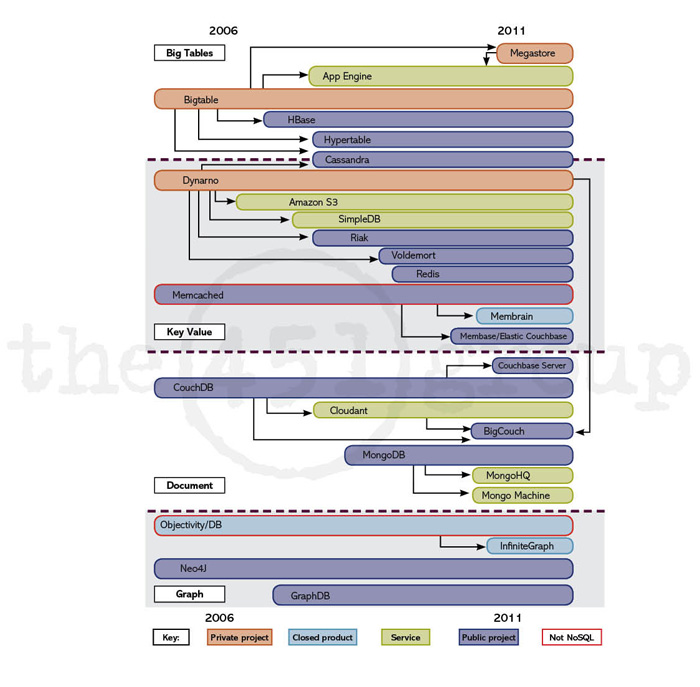
\includegraphics[width=0.5\textwidth]{./kepek/Figures-Aslett2_web.jpg}
\floatfoot{Forrás: \url{http://blogs.the451group.com/information_management/2011/04/}}
\end{figure}

E beszámoló írásakor bátran kijelenthetjük, hogy a NoSQL világ reneszánsz
korszakát éli. Napról, napra újabb és újabb típusú adatbázisok jelenek meg,
amelyek elvetik a relációs adatbázis sémát és valamilyen alternatív adattárolási
struktúra, illetve adat modellezést használva, bizonyos esetekre ideális
adatbázisokat valósítnak meg.  Ezek ősei maradnak a BigTable és Dynamo, ahogy
\aref{fig:NOSQLWorld} ábra szemlélteti is.

Az utóbbi években megfigyelhető, ahogy a NoSQL adatbázisokból származó
tanulságok visszaömlenek a relációs adatbázisok világába megalkotva fél hibrid
rendszereket. Ezeket a szakirodalomban \emph{NewSQL} rendszerekként említik,
kiteljesítve az aktuális adatbázis világképet, ahogyan azt \aref{fig:DBWorld}
ábra is szemlélteti.

\begin{figure}[ht]
\caption{Az adatbázis világ térképe}
\label{fig:DBWorld}
\centering
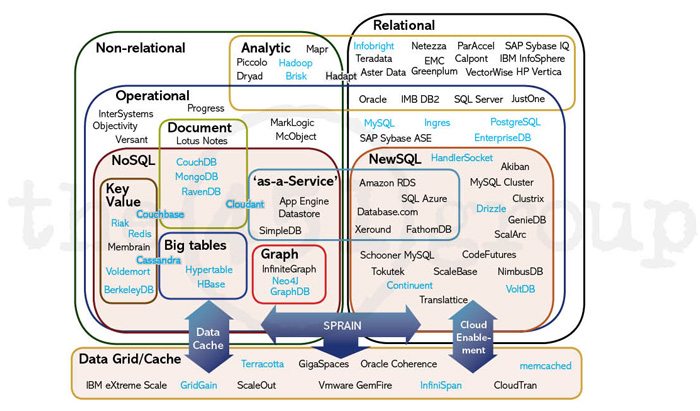
\includegraphics[width=0.5\textwidth]{./kepek/Figures-Aslett_web.jpg}
\floatfoot{Forrás: \url{http://www.the451group.com}}
\end{figure}

\subsection{CAP}

Ha adatbázisok architektúrája után kutatunk, hamar szembesülünk a CAP hármassal.
A CAP az angol \emph{\foreignlanguage{english}{Consistency}}
(konzisztencia),\emph{\foreignlanguage{english}{Availability}} (elérhetőség) és
\emph{\foreignlanguage{english}{Partition Tolerence}} (partíció tolerancia)
szavak rövidítéséből származik. E három fogalmat együtt először $2000$--ben Eric
Brewer vitaindító beszédben használta, mint egy sejtés\cite{Brewer2000}:
szerinte amint alkalmazásaink minél inkább web orientáltak lesznek, annál
kevésbé szabadna az adat konzisztenciára gondolnunk. Az ok, hogy a magas
elérhetőségi szint nem valósulhat meg konzisztencia megkötések betartásával.

Két évvel később Seth Gilbert és Nancy Lynch az MIT--ról ezt formálisan is
bebizonyítót\cite{GilbertLynch2002}, igazat adva Brewernek. De mit is jelent
mind ez? Julian Brown bejegyzésében többet tudhatunk meg\cite{JulianBrowneCAP}.
E szerint, vegyünk egy mindennapi példát. Legyen egy online könyvesboltban egy
könyvből csupán egyetlen példány, továbbá legyen egy \emph{A} és egy \emph{B}
kliens.

\emph{A} érkezik először az oldalra, kosárba teszi a könyvét és tovább
nézelődik. \emph{B} is megérkezik időközbe, kosárba rakja a könyvet és egyből
folytatja is a megrendelési oldallal. A kérdés, hogy hogyan kezeljük a
helyzetet, hiszen evidens, hogy vagy \emph{A} vagy \emph{B} nem fogja tudni
megvenni a könyvet.

Definiáljuk először a CAP három betűjét:

\begin{description}
\item[Konzisztencia] Egy konzisztens rendszerben vagy az egész rendszer működik
vagy semmi. Gilbert és Lynch ezt atomicitás--ként nevezik meg, és ez érhető is,
hiszen azt garantálja, hogy a rendszer soha sem lesz egy átmeneti állapotban.
Bármely művelet egységnyi idő alatt hajtódik végre. Példánk esetében a könyvet
vagy megvesszük, vagy nem. Félig könyvet nem lehet megvásárolni.

Ha mindkettőjük megveheti a könyvet rögtön szembesültünk is egy konzisztencia
szabály megsértésével: a raktárban levő könyv mennyiség, és az eladott mennyiség
különbözik, nincs szinkronban. Erre megoldást jelenthet például, ha a kosárba
tevéskor a raktáron levő könyvek számát csökkentjük, így \emph{B} már nem tudja
a vásárlás műveletet végrehajtani.

\item[Elérhetőség] E szerint az oldal elérhető, azaz betölthető és nem egy hiba
üzenettel tér vissza a böngésző. Ez legtöbb esetben kritikus, hiszen egy nem
elérhető szolgáltatás semmire sem jó.

\item[Partíció tolerancia] Amíg az összes alkalmazás logikát egyetlen gépen
tároljuk addig minden szép és jó. Az elérhetőség szerint vagy fut a rendszerünk
vagy nem. Persze, ez nem mindig egy opció, hiszen így könnyen leterhelhető
rendszerünk és hardver meghibásodások ellen sem vagyunk védve. Viszont amint a
terhet több egységre is leosszuk, partíciók alakulnak ki.

Tegyük fel, hogy két egységre osztottuk le. Amint megszűnik a kommunikációs
lehetőség köztük lehetetlen lesz szinkronban tartani a kettőt. Valahogy azonban
orvosolnunk kell ezt, hiszen a rövid idejű kommunikációs hibák mindennapiak az
elosztott rendszerek világában.
\end{description}

A CAP tétel szerint a fenti három meghatározásból egy időben csak kettőt lehet
megvalósítani. A relációs adatbázisok általában a konzisztencia és az
elérhetőséget válasszák. De a partíció tolerancia forrása a skálázhatóság
megoldása: elosztott rendszerek összmunkája. Ma már tudjuk, egy skálázható
rendszerhez nem minél erősebb, hanem minél több gépet használunk.

Hogy a valós életbeli analógiával éljek, hidat nem egy szuper erős emberrel
húzzunk fel, hanem sok átlagember összmunkájával. A NoSQL világban az, hogy mely
betűt hagyjuk háttérben már nem egyértelmű. \Aref{fig:NoSQLCAP} ábrán láthatjuk,
hogy egy--egy adattároló implementáció a háromszögben hol helyezkedik el.

\begin{figure}[H]
\caption{A CAP hármas}
\label{fig:NoSQLCAP}
\centering
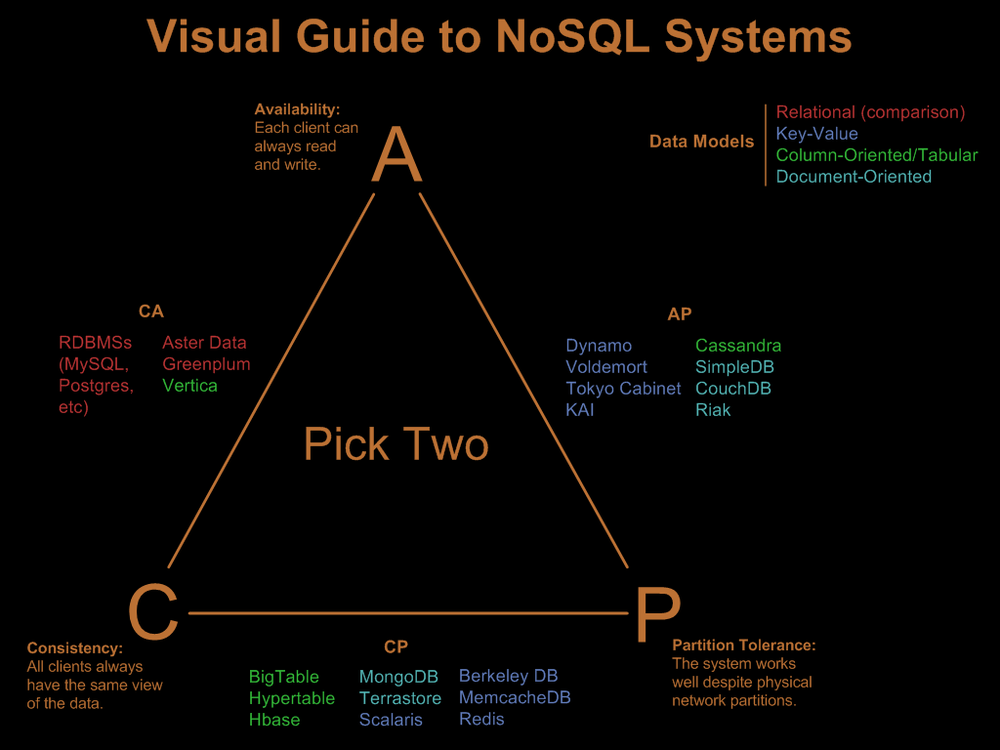
\includegraphics[width=0.7\textwidth]{./kepek/media_httpfarm5static_mevIk.png}
\floatfoot{Forrás:
\url{http://blog.nahurst.com/visual-guide-to-nosql-systems}}
\end{figure}

Az elérhetőség fontossága miatt logikusnak tűnhet, hogy a partíció toleranciáért
a konzisztenciáról mondunk le, de a helyzet nem ennyire komor. A fenti szabály
akkor él, ha az elemek fenti definícióját használjuk. Csupán a konzisztencia
definíciónkon kell kicsit módosítani (lazítani) és akár mindhárom elemet az
asztalon hagyhatjuk. A CAP háromszögre, mint háromszög érdemes gondolni, a
csúcsok a határesetek, amik magukban használhatatlan. Viszont a belsejében
rengeteg átmeneti pont létezik, ami feladatunkra elégséges lehet.

\subsection{Általános struktúra}

A szakirodalomba, főleg Edlich, német professzor,
nyomán\cite{EdlichFriedlandHampeBrauer201010}\cite{Edlich2011}, azon NoSQL
adatbázisok, amelyek adat modelljük főleg oszlop alakban rendeződik ,,széles’’
oszlopcsalád adatbázisnak nevezzük. A név viszont cseppet megtévesztő, mert bár
való igaz, hogy oszlopokat használunk fel, az lényegesen eltér a relációs oszlop
adatbázisok struktúrájától.

Sokkal inkább találó lenne rájuk a táblázatos tároló, avagy a strukturált
kulcs--érték tároló\cite{WideColumnStore}. A korábbi név oly szinten állja meg
helyét, hogy a hagyományos oszlop alapú adatbázisokkal szemben itt lehetséges
(sőt, sokszor ajánlott), hogy egy--egy úgynevezett táblában több millió oszlop
egyidejű létezése is.

\section{Relációs adatbázisok skálázása}
\label{sec:relactios_adatbazis_skalazasa}

Legyen a következő feladat: tervezzünk egy valamilyen szolgáltatást nyújtó
rendszert, amely központi eleme valamely adat tárolása és feldolgozása.
Kezdetben felírjuk az adatbázisunk modellét, az adatokat normalizáljuk táblákban
és a köztük levő kapcsolatokat idegen kulcsok bevezetésével modellezünk. Továbbá
a táblákra indexeket vezetünk be a gyors keresés és szűrés érdekében. Ha több
táblából kiszámítható adat érdekel valószínűleg végre fog kelleni hajtanunk egy
vagy több JOIN művelet az SQL lekérdezés kiértékelésére.

Továbbá az adatbázisunk robusztussága érdekében felhasználjuk a relációs
adatbázisok olyan funkcionalitásait mint a \emph{tárolt eljárások}. Ennek
segítségével garantálni tudjuk, hogy ha még több forrásból is egy időben
frissítünk adatott, adatbázisunkban a különböző táblák adatai mindig
megegyeznek, sose mondanak ellent egymásnak. A \emph{tranzakciók} lehetővé
teszik, hogy akár több tábla adati frissítését is mind egy atomos, egységnyi
művelet hajtsuk végre.

A relációs adatbázisok biztosítják az ACID tulajdonságokat, amelyek egy erős
konzisztenciát tesznek lehetővé az adatbázis keretén belül. Továbbá az
\emph{SQL} nyelvvel deklaratív módon általános lekérdezéseket fogalmazhatunk
meg. Az \emph{alkalmazás séma} eltakarja, elölünk, hogy a háttérben pontosan
hogyan is van tárolva az adat. Lehetővé teszi, hogy az adataink felhasználására
összpontosítsunk a tárolási adatstruktúrák helyet.

Rendszerünk futtatásában mindez elég hosszú ideig jól szolgál. Azonban, amint
egyre több és több felhasználó csatlakozik szolgáltatásunkra ara leszünk
figyelmesek, hogy adatbázisunk egyre jobban le van terhelve. Az első lépés e
terhelés csökkentése felé, hogy szolga szervereket iktatunk be. Ezeket csak
párhuzamos olvasásra használjuk. Továbbra is egyetlen mester adatbázis van,
amely fogadja az összes beérkező írást. Az alkalmazások nagy részében az írások
száma jócskán alacsonyabb az olvasások számával, így ez egy könnyű kiút lehet a
problémából.

Viszont, ha a szolgáltatásunk még népszerűbb lesz, eljutunk azon pontra, hogy
már ez sem segít. Ekkor beiktathatunk egy cache--elő rendszert, mint például a
Memcached. Most már az olvasást egy nagyon gyors, memória alapú rendszer
szolgálja ki, de cserében elveszítünk az erős konzisztencia garanciánkat, mert a
memória és a háttér tároló között eltérések fordulhatnak elé. De ez nem add
megoldást a sok párhuzamos írásra.

A függőleges skálázás az egyetlen biztos eszközünk: több magos processzor, több
memória és gyorsabb háttér-tároló. De ez igencsak drága lehet, főleg ha a
korábbi mester--szolga architektúrát már alkalmaztuk, hiszen a mester és a
szolgák egyforma erősnek kell lennie. Ellenkező esetben előfordulhat, hogy a
szolga nem képes tartani a lépést a mesterrel.

A szolgáltatás fejlődésével egyre több új funkció iránti igény merül fel,
amelyek kiszolgálása valószínűleg akár komplex JOIN műveletek végrehajtását is
igényeli. Ami ugyanakkor még több adatbázis lekérdezés megjelenését jelenti. E
pontban a JOIN műveletek már igen költségesek, és a tábláinkat denormalizálni
kell, hogy elkerüljük e költséget.

Ha minden szakad a tárolt eljárásokat is ki kell kapcsolnunk, hiszen akár már
ezek is túl sok ideig futnak. E fázisban már az adatott nem úgy tároljuk, hogy
azt kényelmes legyen feldolgozni, hanem a használt lekérdezésekhez
optimalizálva.

A következő lépés, hogy a gyakran bejövő komplex lekérdezéseket idő előtt
lefuthatjuk (korai materializáció). Végezetül az indexek vezetését is
kikapcsoljuk, mivel már ezek karbantartása is igen költséges művelet a leterhelt
adatbázisunk számára. Ha forgalmunk még tovább növekedhet muszáj lesz
adatbázisunk részekre leosztani (sharding), de ez egy adminisztrációs fejfájás
és igencsak nehéz jó, könnyen skálázható módon kivitelezni. Már
\aref{fig:DatabaseShard} ábrán szemléltet egyszerű leosztás megvalósítása is
probléma dús és hosszas művelet lehet.

\begin{figure}[H]
\caption{Adatbázis feltördelése darabkákra}
\centering
\label{fig:DatabaseShard}
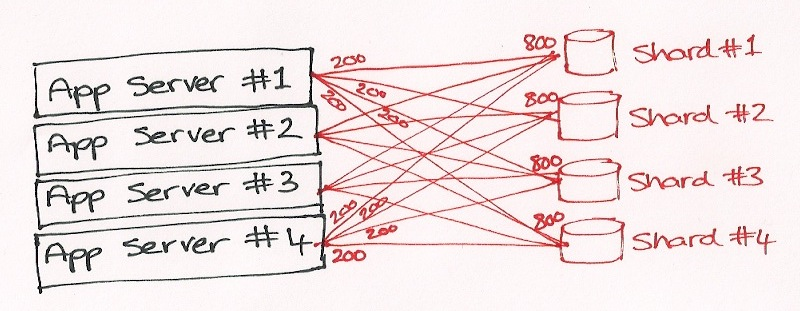
\includegraphics[width=0.5\textwidth]{./kepek/ShardDiagram-4.jpeg}
\floatfoot{Forrás: \url{http://www.dbshards.com/articles/database-sharding-configuration/}}
\end{figure}

Mindez azt mutatja, hogy a relációs adatbázisok felépítésük miatt nehézkesen
skálázhatóak. Ne értsük félre, a relációs adatbázisok még mindig a legjobb és
legkényelmesebb megoldást szolgálják egy adott szintig. A kérdés az, hogy ha
tudjuk, hogy ezt a szinten túl lépjük egy idő után, nem lenne értelmesebb egy
olyan architektúra mentén elindulni, amely mindezt könnyedén megvalósítja? Egy
ilyen megoldás lehet a NoSQL oszlop alapú adatbázisok.
 
\chapter{Implementációk}
A NoSQL alapú oszlopcsaládok között két implementációnak sikerült széles körű
ipari használhatott elérni: a Cassandra és a HBase. Mindkettő Apache projekt.
Architektúrájukban megfigyelhető kiinduló pontjuk, a Google BigTable és az
Amazon Dynamo közötti különbség. Míg az első a meglévő Google fájl rendszere
épít és kihasználja az általa nyújtott absztrakciós szintet (szolgáltatásokat),
addig a későbbi önállóan is működő képes rendszer. Ennek megfelelően az összes
problémát saját maga próbálja megoldani.

\section{Apache Cassandra}
A Cassandrát a Facebook fejlesztette, első körben, mint skálázható adattároló a
szociális hálójához. Az első fejlesztők között volt az Amazon Dynamo
megalkotója, Avinash Lakshman\cite{Lakshman:2010:CDS:1773912.1773922}, így
nem meglepetés, hogy főleg annak architektúráját és elképzelését követi. $2008$
júliusában a forráskód nyílttá vált, a Google Code web felületen keresztül.
$2009$ márciusában a projekt az Apache projekté alakul át. $2010$ februárjában
pedig fő szintű projekté alakul át az Apache szervezet keretében. Licensze ennek
megfelelően az Apache Licensz $2.0$\cite{CassandraManual}.

\begin{center}

\includegraphics[width=0.3\textwidth]{./kepek/Cassandra_logo.png}
\end{center}

Két kulcs pontja van egy Cassandra rendszernek: az adat partíció és az adat
modell.

\subsection{Adat partíció}

A Cassandra egy elosztott alapú adattároló rendszer. Ez azt jelenti, hogy
egyszerre több számítógépen is futhat ugyanazon adattároló példány. Ebből
következik, hogy az egyik feladat az adatok leosztása a rendszer egy-egy gépére.
Induljunk ki egy adathalmazból, amint tárolni szeretnénk. Tegyük fel, hogy ez
már valamilyen logika szerint el van osztva. Beérkezik egy új adategység a
klienstől, a rendszer egy adott gépéhez. Kérdés: hova rakjuk az új adategységet,
hol tároljuk el, hogy később könnyedén megkapjuk? A helyzetet ábrázolja
\aref{fig:WhereToStore} ábra.

\begin{figure}[ht]
\caption{Adat halmaz tárolása klaszter felett}
\centering
\label{fig:WhereToStore}
\includegraphics[width=0.5\textwidth]{./kepek/adat_tarol.png}
\end{figure}
	

A Cassandra válassza erre az \emph{adat gyűrű}. Ennek egy sematikus felépítését
\aref{fig:CassandraDataRing} ábra szemlélteti. Minden adat egységnek van egy sor
azonosítója, ez alapján számolódik rá egy \emph{MD$5$} hash érték. A gyűrű e
hash értelmezési intervallumot osztja le a gépekre. Minden rendszerbe résztvevő
gép kap egy értéket a hash intervallumból. Így a gépek egy kört alkotnak, mivel
a legmagasabb hash értéket kapó gépet a legkisebb értékű követi.

\begin{figure}[ht]
\caption{A Cassandra adat gyűrű}
\label{fig:CassandraDataRing}
\centering
\begin{tikzpicture}[scale=1.7]
 \tikzset{
  cassandraNode/.style={circle,green,fill=green,minimum width=0.15},
  cassandraToken/.style={rectangle, rounded corners, red, fill=green}
  }
  %\draw[help lines] (-3,-3) grid (3,3);
  % the big circle
  \draw[blue,thick, fill=bgSrc] (0,0) circle [radius=2cm] ;
   % draw splitting lines
  \draw (0,-2) -- (0,2);
    % draw splitting lines
  \draw (-2,0) -- (2,0);
  
  \node[cassandraNode] (cT) at (0,2) {};
  \node[cassandraNode] (cL) at (-2,0) {};
  \node[cassandraNode] (cR) at (2,0) {};
  \node[cassandraNode] (cB) at (0,-2) {};
  
  \node[cassandraToken] (rT) at (0, +2.4) {0};
  \node[cassandraToken] (rR) at (2.4, 0) {25};
  \node[cassandraToken] (rB) at (0, -2.4) {50};
  \node[cassandraToken] (rL) at (-2.4, 0) {75};
  
  \draw[-] (rT) -- (cT);
  \draw[-] (rL) -- (cL);
  \draw[-] (rR) -- (cR);
  \draw[-] (rB) -- (cB);
  
  \node[circle, green, red, fill=yellow, minimum width=.1] (cE) at
  (1.73, -1) {};
  \node[] (lE) at (2.2, - 1.5)  {30-as sor}; 
  \draw[<-] (cE) -- (lE);
  \draw[->, densely dashed] (cE) .. controls (1, -2.5) .. (cB) node
  [draw=none,midway,below=0.1] {Replikáció};
  % Legend
  \node[rectangle, align=center] (f) at (3, 0.7) {Adat \\csomópont};
  \node[rectangle, align=center] (g) at (-3, 0.7) {Csomópont\\token};
  \draw[<-] (2.12,0.1) -- (f);
  \draw[<-] (-2.4,0.2) -- (g);
  
  % direction circle
  \draw[blue,<-] (-2.1,-1.8) .. controls (-2.75,-1.9) and (-2.1, -2.8)..
  (-2, -1.9) node [black,draw=none,midway,below=0.1] {írány a gyűrűn};
   
\end{tikzpicture} 
\end{figure}

Egy adott gép azon adat bejegyzéseket tárolja, amik az ő és előtte levő hash
érték intervallumba tartozik. A helyzet kicsit tovább bonyolódik, amikor
redundancia is bejön a képbe; hiszen most már nem csak egy helyre, hanem több
gépre is ki kell írnunk ugyanazon adatott.

A Cassandra ebben az esetben a gyűrűn tovább haladva, az éppen beállított
replikációs szint szerint, következő \emph{n} fizikai egységre is kiírja az
adatott. A konkrét egységek kiválasztásakor számításba vehet az adattárházak
fizikai struktúráját is. Így biztosítva, hogy amennyiben még az egész tárház is
kiesik egy másikba egy gépen mindig elérhető lesz a szükséges adat.

A gyűrűből az írás és olvasás a lehető legjobb teljesítmény elérésének érdekében
futás időben konfigurálható. Rendelkezésünkre állnak oly módszerek, mint
\emph{egy}, \emph{kettő}, \emph{három}, \emph{bármely}, \emph{mindegyik} avagy
\emph{lokális kvórúm}. Az utolsó mód akkor lesz létfontosságú mikor földrajzilag
egymástól távoli adat tárházakat rakunk egy rendszerbe.  Legyen például egy
online üzletház, amely világ szinten üzemel és szállít. Természetes elvárás,
hogy a magyar országi klienseknek a szolgáltatás ugyanolyan jól működjön, mint
az Egyesült Államokban.

Viszont ennek megvalósításába beleütközünk a fénysebességből adódó adat átvivő
késleltetési időbe, amely $100$ms feletti egy óceánon keresztüli útvonalon.
Alkalmazás és adatbázis szervereink nem lehetnek sem csak Magyarországon, sem
csak az Egyesült Államokban, hiszen a túloldalon a szolgáltatás jóval lassabb
lenne, és ennek megfelelően gyengébb élményt nyújthat. Megoldás, hogy mindkét
kontinensen elhelyezünk egy--egy klasztert és egy adott kérés kiszolgálásához
lehetőleg csak a földrajzilag helyit használjuk fel.

Ilyenkor a lokális döntő képesség (kvórum) opcióval azt biztosíthatom, hogy a
lekérdezett adat a helyi adattárház szintjén konzisztens. A kvórum a létező
egységek felét plusz egy számát jelenti, tehát egy $5$ egységből álló Cassandra
hálózat esetében legalább $3$ ugyanazzal az érték válasszal tér vissza. A
lokális kvórum ennek megfelelően például a magyarországi Cassandra gépek fele
plusz egytől várja el ugyanazt a választ. Amint ez megtörtént a kliensnek
visszatéríti a kapott adatott.

Ez gyakran elégséges, hiszen elég kis arányban fordul elő, hogy egy--egy kliens
kiszolgálására globális nézetre van szükségünk, hiszen például az amerikai
rendelés kiszolgáláshoz csupán az amerikai készlet szükséges. Ugyanakkor, ha
globális jelentéseseket, elemzéseket kívánnunk futtatni a lehetőség megvan.
Mivel rendszerünk a globális olvasási kéréssel még egyként látható.

\subsection{Adat modell}

Az adat modell lényegben eltér a relációs adatbázisoktól. Mi több, szerintem e
rendszerekben megfordul a hagyományos relációs adatbázisok használati
munkamenete. A relációs adatbázisokra jellemző, hogy strukturáljuk és
rendszerezzük a rendelkezésünkre álló adatot, majd különböző főleg JOIN
műveletek használatával a kért információt SQL nyelv segítségével kérjük le.
Mikor egy Cassandra rendszert használunk a JOIN és az SQL--t is felejtsük el.
Habár létezik egy SQL--re emlékeztető CQL (Cassandra Query Language) ez nem
támogat JOIN műveleteket.

Ebből adódóan, egy jól működő rendszerbe nem az adatbázisunkban levő adatott
rakjuk össze, hogy kinyerjünk valamilyen információt, hanem úgy tervezzük meg
adatbázisunkat, hogy könnyű legyen azt lekérdezni. Még akkor is, ha emiatt
egy--egy adatott többször is el kell tárolni. A cél a gyors és hatékony
lekérdezés, amely érdekében az olcsó merevlemez tár mennyiséggel vagyunk
hajlandóak fizetni. Egy Cassandra adatbázis megalkotása nem úgy kezdődik, hogy
milyen adatunk van, hogy tároljuk el; hanem, hogy milyen lekérdezéseket akarunk
majd elvégezni?

A relációs adatbázisok belli sémák kulcs téré módosulnak, a táblák oszlop
családokká. A hasonlat viszont itt megáll, mert nincs idegen kulcs, nincs
kapcsolat a családok között és olvasás közben nem lehetséges a családokon JOIN
művelet. Ennek megfelelően, ha valamilyen adat szükséges egy lekérdezéshez,
akkor annak ott kell lennie az oszlop családban, mint egy oszlop.

Az oszlop családok oszlopokból állnak. Egy oszlopcsalád lehet \emph{statikus}
vagy \emph{dinamikus}. Az oszlopok meg a következő típusok közül vehetnek fel
egyet: \emph{standard}, \emph{összetett}, \emph{lejáró}, \emph{számláló} avagy
\emph{szuper}.

\subsubsection{Oszlop család típusok}

 \paragraph{Statikus} 
 
Az egyszerűbb, többé--kevésbé megfelel a relációs adatbázisok tábláinak, itt is
az oszlopcsalád oszlopait előre definiáljuk és a futás időben beszúrt értékeknek
e struktúrát követnie kell. \Aref{fig:CassandraColumnFamiliyStatic} ábra például
egy felhasználó adatait tároló oszlopcsaládot mutat.

Abban viszont eltér a relációs tábláktól, hogy nincs szükség NULL elemre a
hiányzó adat mezők (oszlopok) jelzésére. A Cassandra oszlopcsaládok natív módon
képesek úgy nevezett ritka tárolásra. Amely oszlop nem létezik az oszlop
családból, azt egész egyszerűen nem vesszük fel a sor beszúrásakor.
 
\begin{figure}[H]
\caption[Statikus oszlopcsalád a Cassandrában]{Statikus oszlopcsalád a
Cassandrában\cite{CassandraManual}
}
\centering
\label{fig:CassandraColumnFamiliyStatic}
 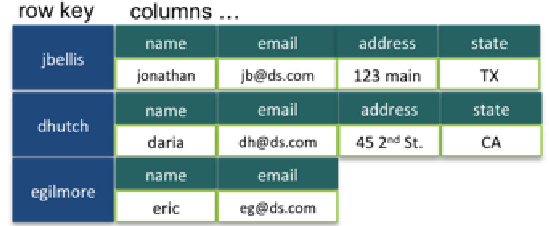
\includegraphics[width=0.3\textwidth]{./kepek/simple_column.png}
\end{figure}

\paragraph{Dinamikus} 
 
Ez esetben akár az oszlop név maga is jelentheti az adatott, és így ezt a kliens
futásidőben szolgáltatja, a Cassandra meg dinamikusan hozza létre. 
Funkcionálisan úgy lehet felfogni, mint egy előre materializált nézetet, amelyet
előre kiszámolunk, és hatékony módon tárolunk el. Ez esetben csak az oszlop név 
és tartalmának típusát kell előzetesen definiálni. 
\Aref{fig:CassandraColumnFamiliyDynamic} ábra például felhasználók közti
kapcsolatot modellez egy oszlop családba foglalva mindezt.
 
 \begin{figure}[H]
\caption[Dinamikus oszlopcsalád a Cassandrában]{Dinamikus oszlopcsalád a
Cassandrában\cite{CassandraManual}
}
\centering
\label{fig:CassandraColumnFamiliyDynamic}
 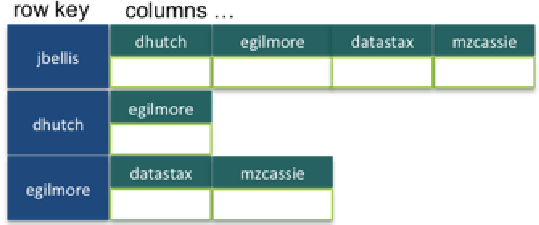
\includegraphics[width=0.3\textwidth]{./kepek/dynamic_column.png}
\end{figure}
 
\subsubsection{Oszlop típúsok}
Az oszlop a legkisebb adat elem a Cassandrában: egy név, érték és egy
időbélyeg páros.
 
\paragraph{Statikus} 

Az oszlopnak egy névvel kell rendelkeznie, amely lehet: statikus, avagy
dinamikus (attól függően, hogy előre definiált, avagy futás közben hozzuk
létre). Egy oszlopnak az értéke fakultatív. Az időbélyeg megadható, avagy
amennyiben hiányzik a beszúrás pillanatbeli időbélyeggel lesz ellátva.
Olvasáskor mindig csak a legújabb érték lesz visszatérítve (hacsak explicit nem
kérünk egy régebbit).

 \begin{figure}[H]
\caption[Oszlop struktúra a Cassandrában]{Oszlop struktúra a
Cassandrában\cite{CassandraManual}
}
\centering
\label{fig:CassandraColumnStandard}
 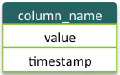
\includegraphics[width=0.1\textwidth]{./kepek/standard_column.png}
\end{figure}

\paragraph{Összetett}
Az összetett csoportok egy újabb absztrakciós szintet vezetnek be és
segítségükkel klaszterezett sorokat lehet tárolni. Az összes logikai sor, amely
partíciós kulcsa ugyanaz lesz, egyetlen széles sorként lesz eltárolva. Így egy
sorba akár 2 milliárd oszlop is lehet. Az összetett oszlop segítségével a
sorokat teljesen denormalizálható egy előre definiált összetett kulcsot
felhasználva.

Legyen egy tweet alkalmazás, ahol az adathalmazhoz tartozik a bejegyzés szövege,
felhasználó név és azok követő listái. A feladat, hogy gyűjtsük össze egy adott
felhasználó követőinek bejegyzéseit. Ehhez hozzuk létre először egy \emph{tweet}
táblát, amelybe bejegyzéseket tárolunk felhasználókhoz. Generáljunk
automatikusan minden bejegyzéshez egy azonosítót. \Aref{tab:tweetTable} tábla
egy példa bejegyzést mutat.

\begin{minted}[numbersep=5pt,
                gobble=0,
                frame=lines,
                framesep=2mm,
                bgcolor=bgSrc]{sql}
 CREATE TABLE tweets (
 tweetid uuid PRIMARY KEY,
 author varchar,
 body varchar
 );
\end{minted}

\newcolumntype{g}{>{\columncolor{bgSrc}}l}
\begin{table}[ht]
\begin{tabular}{g|c|r}
\hline \rule[-2ex]{0pt}{5.5ex} 
tweet\_id & author & body \\ 
\hline 
1 & A & XY \\
2 & B & YZ \\
3 & C & ZT 
\end{tabular} 
\caption{Egy tweet oszlopcsalád}\label{tab:tweetTable}
\end{table}

A tweet táblát denormalizáljuk, az összetett oszlopok az összetett fő kulcs
szerint valósul meg:

 \begin{minted}[numbersep=5pt,
                gobble=0,
                frame=lines,
                framesep=2mm,
                bgcolor=bgSrc]{sql}
 CREATE TABLE timeline (
 userid varchar,
 tweetid uuid,
 author varchar,
 body varchar,
 PRIMARY KEY (userid, tweetid)
 );
 \end{minted}

A két azonosító együtt azonban szükséges is, hiszen magára egyik sem lenne
egyedi. \Aref{tab:timelineTable} tábla ad erre is egy példát. A két tábla
felépítését \aref{fig:timelineTweetFigure} ábra szemlélteti. A háttérben
továbbra is csak egy fő kulcs lehetséges. Ezért, az összetett kulcs első eleme
lesz a partíciós kulcs. Az dönti el, hogy az adat gyűrűben a bejegyzés hova
kerül. A kulcs maradék része szerint klasztereződnek az illető sorba bejegyzett
elemek.

A klasztereződés abban valósul meg, hogy a tároló motor létrehoz egy indexet, és
mindig a szerint tárolja az adatott. Mivel a felhasználó név az adat partíciót
megvalósító kulcs, a maradék kulcs (a tweet id) szerint lesz rendezve a többi
bejegyzés. \Aref{tab:timelineTable} példa esetében a háttérben
\aref{tab:compositedColumn} módon lesz eltárolva.
 
\begin{table}[ht]
\centering
\begin{tabular}{g|g|c|r}
\hline \rule[-2ex]{0pt}{5.5ex} 
user\_id & tweet\_id & author & body \\ 
\hline 
D & 2 & B & YZ \\
D & 1 & A & XY \\
E & 4 & C & ZT \\ 
E & 1 & A & XY 
\end{tabular} 
\caption{Egy timeline oszlopcsalád}\label{tab:timelineTable}
\end{table}

\begin{figure}[H]
\begin{tikzpicture}
  [->,scale=.8,auto=left,every node/.style={circle,fill=blue!20}]
  \node (A) at (3,2) {A};
  \node (B) at (1,2)  {B};
  \node (C) at (5,2)  {C};
  \node (D) at (2,1) {D};
  \node (E) at (4,1)  {E};
  \node[style={scale=.7}] (1) at (3,4) {1-XY};
  \node[style={scale=.7}] (2) at (1,4) {2-YZ};
  \node[style={scale=.7}] (3) at (5,4) {3-ZT};

  
    \draw (D) -> (B);
    \draw (D) -> (A);
    \draw (E) -> (A);
    \draw (E) -> (C);
    
     \draw (A) -> (1);
     \draw (1) -> (A);
     \draw (B) -> (2);
     \draw (2) -> (B);
     \draw (C) -> (3);
     \draw (3) -> (C);

\end{tikzpicture}
\caption{A tweet és timeline tábla felépítése}\label{fig:timelineTweetFigure}
\end{figure}


\begin{table}[ht]
\begin{tabular}{g|c|c|c|c}
\hline \rule[-2ex]{0pt}{5.5ex}
D & [2,author]:B & [2,body]:YZ  & [1,author] : A & [1,body] : XY \\
E & [4,author]:C & [4,body]:ZT  & [1,author] : A & [1,body] : XY \\  
\hline
\end{tabular} 
\caption{Egy összetett oszlop példa tárolása}\label{tab:compositedColumn}
\end{table}

Ezen táblákkal egy adott felhasználó követőjének a tweet listájának lekérdezése
CQL nyelvben:

 \begin{minted}[numbersep=5pt,
                gobble=2,
                frame=lines,
                framesep=2mm,
                bgcolor=bgSrc]{sql}
   SELECT * FROM timeline WHERE userid = D 
            ORDER BY tweetid DESC LIMIT 50;
 \end{minted}

Láthatjuk, hogy habár a háttérben a Cassandra alapjában eltér a relációs
adatbázisoktól, formailag a CQL igyekszik követni az SQL nyelvet.

\paragraph{Lejáró oszlopok}
Bármely oszlophoz hozzácsatolhatunk élettartamot, angolul:
\foreignlanguage{english}{Time to live - \emph{TTL}}, amelyet beszúráskor lehet
beállítani. Amint ez lejár az oszloptörlésre megjelölve lesz. Ez azt jelenti,
hogy lekérdezéskor már nem számit. Törölve viszont még nem lesz. Az csak a
periodikus csomagolási műveletek elvégzésekor történik meg.

A Cassandra rendszerben egy elem beszúrása beszúrás amennyiben az oszlop elem
még nem létezik, egyébként meg frissítés. Oszlop élettartamot frissíteni nem
lehet, de hasonló hatást érhetünk el, ha kiolvassuk az elemet, majd ismét
beszúrjuk új lejárati idővel. A lejárati idő bekapcsolása természetesen további
$8$ bájt merevlemez és memória költséggel jár.

\paragraph{Számláló oszlopok}

Egy számláló oszlop speciális oszlop családot igényel, e miatt gyakorlatilag
saját oszlopcsaládot kell létrehozni. Ellenben, amint ez megtörtént egy--egy
számláló érték frissítésére csupán a változási értéket kell megadnunk.

\begin{itemize}
\item[\smiley] Működik elosztott rendszerekbe.
\item[\frownie] A Cassandra szerverek órái szinkronban kell, hogy legyenek a
helyes működéshez.
\item[\frownie] Íráskor elégséges az egy írási parancs, de mivel a rendszer a
számlálókat konzisztensnek kell, hogy tartsa a háttérben egy globális olvasási
művelet is végre fog hajtódni.
\end{itemize}

\paragraph{Szuper oszlopok}
Ezek egy extra absztrakciós szintet vezetnek be, az oszlop és az oszlop család
közzé. Sajnos csak kis oszlop szám mellet működik hatékonyan ezért helyettük az
összetett oszlopok használata ajánlott.

\subsection{Adat típusok}
Típusa lehet az oszlop értékének (érvényesítő) és az oszlop nevének
(komparátor).

\begin{description}
  \item[Érvényesítő] Meghatározza, hogy az érték beszúrható e vagy sem ebbe az
  oszlopba. Bármikor újra definiálható.
  \item[Komparátor] Meghatározza, hogy az oszlop név helyes e (dinamikus
  oszlopcsalád esetében) és az oszlop családban az oszlopok eszerint kerülnek
  rendezésre. Definiálás után többet nem változtató meg, tehát gondoljuk meg
  alaposan, hogy mit választunk.
\end{description}

\subsection{Oszlopcsalád tervezési tanácsok}
Kezdjük azzal, hogy megfogalmazzuk, hogy milyen információk érdekelnek.
Gondoljuk el, hogy hogyan tudjuk ezeket lekérdezni. Minden adat, ami egy
lekérdezéshez szükséges tegyük egy oszlop családba, de ne rakjuk mindent egy
oszlop családba. Ha egyes adatott többször is eltárolunk az nem gond, a
Cassandra nézőpontjából a tárhely olcsó. Cserébe gyors lekérdezéseket kapunk.

Gondoljuk meg, ha szükségünk van generált egyedi azonosítóra, avagy az
természetesen adódik. A természetes kulcs tulajdonságai:

\begin{itemize}
\item[\smiley] A tárolt adatot szabad szemmel is könnyedén olvasható.
\item[\neutranie] Elkerüljük a denormalizációs műveleteket és az index
alkalmazásának szükségességét.
\item[\frownie] Nem lehet megváltoztatni a kulcsot. Tehát például a felhasználó
nevet miután létrehoztuk többet nem lehet megváltoztatni.
\item[\frownie] Az alkalmazás garantálja a kulcs egyediségét. Ha ez valamiért is
sérülne felülírhatjuk az adatott.
\end{itemize}

A Cassandra rendszer egységnyi (aqtomikus) sor műveletek szintjén. Íráskor és
olvasáskor is specifikálhatjuk, hogy milyen konzisztencia szintet óhajtunk.
Általában a Cassandra egy előbb--utóbb konzisztens rendszer, ami szerint, ha egy
ideig nem történek új elem beszúrások a rendszer automatikusan beáll konzisztens
állapotba. De a konzisztens állapot sosem garantált, tehát gondoljuk meg, hogy
milyen szintű lekérdezéseket kérünk.

\newpage
\section{Apache HBase}
\begin{center}

\includegraphics[width=0.3\textwidth]{./kepek/hbase_logo.png}
\end{center}
A HBase a Cassandrához hasonlóan ugyancsak felső szintű Apache projekt. Gyökerei
$2003$--ban indult a Google--nál a Google File System\cite{googlefilesystem}
megalkotásával. Célja volt egy olyan rendszer megalkotása amely:

\begin{itemize}
\item[\smiley] Egy olcsó és könnyen beszerezhető hardver klasztere támaszkodik.
\item[\smiley] Képes óriás mennyiségű adat eltárolására.
\item[\smiley] Belsőleg megoldja az adat replikációt a klaszter pontjai között.
\item[\smiley] Adat folyam áramlatú olvasásra optimalizált.
\end{itemize}

Miután mindezt sikerült készült el csakugyan a Google--nál a
MapReduce\cite{dean2008mapreduce} amely egy \emph{egyszerűsített adatfeldolgozó}
amely képes nagy klaszter farmok felett is hatékonyan működni. A GFS + MapReduce
páros most már:
\begin{itemize}
\item[\smiley] Az adat feldolgozáshoz hasznosítjuk az adat tárolásra.
már úgyis meglevő fürt processzor készletét.
\item[\smiley] Hatékony pár nagyméretű fájl kezelésére.
\item[\neutranie] Nem biztosit véletlenszerű adat elérést közel valós idősbben.
\item[\frownie] Nem teszik lehetővé akár több millió apró fájl kezelését. E
mögött az egyik ok, hogy egy--egy számítógép csak véges számú fájlt nyithat meg
egyszerre.
\end{itemize}

De a Google Mail és Analytic termékük pont sok kis fájl használatát igényelte.
Ezért a kutatás egy olyan adattároló terelődött, amely felhasználja a már
meglevő infrastruktúrát, képes kis entitások tárolására és ezt a háttérbe nagy
fájlokká rakja össze (így belefér a GFS--be). A gyors véletlenszerű merevlemez
elérés érdekében valamilyen indexelési stratégiát vettünk be. Ugyanakkor
használja fel a MapReduce--t is mint elosztott adatfeldolgozó rendszer.

Ehhez először is a Google lemondott az adattárház relációs jellegéről, majd öt
kulcs fontosságú műveletre gyúrt: \emph{írás} (create), \emph{olvasás} (read),
\emph{frissítés} (update), \emph{törlés}(delete) és \emph{felderítés}(scan). Az
eredményt 2006--ban a BigTable cikkben\cite{Chang2006} tárgyalták: létrehoztak
elosztott tároló rendszert strukturált adathalmazra. A rendszer fő
tulajdonságai: az elosztottság, az adat lehet szórványos (ritka), perszisztens
és több dimenziós rendezett szótár.  Egy évvel később innen kiindulva alakult
meg a HBase (Hadoop Database).

\subsection{Adat modell}
Az alap építőelem az oszlop\cite{hbase2011george}. Egy vagy több oszlop egy
sort alkot. A sort egyértelműen megcímez egy egyedi azonosító. A sorok egy
halmaza táblát alkot. Minden oszlopnak lehet több verziója, egy--egy ilyenre, 
mint cella vonatkozzunk. Két cellát egymás között egy automatikus vagy
felhasználó által szolgáltatott idő bélyeg különböztet meg.

A sorok mindig lexikografikus módon vannak rendezve a kulcsuk szerint. Érdemes
megemlíteni, hogy e miatt a számok nem numerikus sorrendbe lesznek rendezve.
Például a $10$ a $2$ előtt jön. Amennyiben számokat akarunk rendezni, azokat
egészítsük ki nullákkal, azaz $2$ helyet $02$--öt rendelünk hozzá a sor
kulcsához. Két kulcs összehasonlítása bájt szinten történik, az első különböző
bájtnál az összehasonlítás leáll. Így a sor kulcsa a relációs adatbázisokban már
megismert fő indexként viselkednek.

Az oszlopok továbbá oszlop családba csoportosíthatók. Szerepük, hogy rengeteg
HBase által szolgáltatott funkció oszlopcsalád szinten konfigurálható. Ilyen
például az alkalmazott sűrítési metódus. De például az oszlopcsalád oszlopai
mindig ugyanazon fájlba tárolódnak, így az oszlopcsaládok elvégzett lekérdezés
elvégzéséhez biztos, hogy legfeljebb csak egy fájlt kell beolvasnunk egy adott
gépen a merevlemezről.

A HBase által használt fájlt HFile--nak nevezzük, és perszisztens, illetve
változhatatlan. A fájl tartalma a kulcs szerint rendezve van. A fájl egy blokk
szekvencia, amelynek az indexe alkotja az utolsó blokkot. Így egy sor
kiolvasásához legfeljebb két művelet szükséges. Egy, amelyik beolvassa az index
blokkot és egy, amely az index szerint a következő sort. Az index blokk viszont
bekerül a memóriába ekkor és a következő lekérdezésekkor már csak a sort kell
beolvasnunk.

Az oszlop családokra igaz, hogy:
\begin{itemize}
  \item[\smiley] A család belsejében az oszlop számra nincs korlát.
  \item[\neutranie] Struktúrája \emph{család:minősítő} alakú.
  \item[\neutranie] Definiálni kell a tábla létrehozásakor.
  \item[\neutranie] Ritkán változnak.
  \item[\frownie] Neve nyomtatható kell, hogy legyen.
  \item[\frownie] Csupán pár tíz használható fel belőle, ha hatékonyan működő
  rendszert óhajtunk.
\end{itemize}

A cella értéke bájt sorozat formájában tárolódik. Annak értelmezése a
felhasználó alkalmazás feladata. Egy HBase adat elérési útvonalát megadhatjuk,
mint:

\begin{displaymath}
(\text{Tábla}, \text{Sor Kulcs}, \text{Oszlop család}, \text{Oszlop}
\text{\emph{,Idő bélyeg}}) \mapsto \text{Érték}
\end{displaymath}

Ami adat struktúra szinten: 

%  \begin{minted}[numbersep=5pt,
%                 gobble=2,
%                 frame=lines,
%                 framesep=2mm,
%                 bgcolor=bgSrc]{python}
    \begin{verbatim}
   Map<Row, List < Map <Column, List<Value, Timestamp> > >
   \end{verbatim}
%  \end{minted}
 
\subsection{Adat partíció}
A partíció központi eleme a régió. A régió nem más, mint egy folytonos sor
halmaz, amely egy helyen van tárolva. Kezdetben egyetlen régió létezik. Amint
egy régió átlépi az előre definiált határokat (írás, olvasás) a régió közepénél
fogva automatikusan kettéválik, két új régióra. Két régió összes is olvadhat, ha
azoknak mérete és kihasználtságuk kicsi lesz.

A régiók \emph{régió szervereken} helyezkednek. Egy régió szerveren akár több
régió is helyet kaphat, viszont egy régió csak egy régió szerveren fordul elő.
Például attól függően, hogy milyen betűvel kezdődik a sor kulcsa
\aref{fig:regionServer} ábrán láthatunk egy lehetséges leosztást.

\begin{figure}[ht]
\begin{tikzpicture}
  [->,scale=.8,auto=left,every node/.style={fill=blue!20}]
  \node (reg1) at (1,3) {A-I régió};
  \node (reg2) at (1,2)  {I-N régió};
  \node (reg3) at (1,1)  {N-W régió};
  
  \node (szerv1) at (5,    2.5)  {Régió szerver 1};
  \node (szerv2) at (5,  1)  {Régió szerver 2};
  
  \draw (reg1) -> (szerv1);
  \draw (reg2) -> (szerv1);
  \draw (reg3) -> (szerv2);
  
\end{tikzpicture}
\caption{Régiók és régió szerverek}\label{fig:regionServer}
\end{figure}

Egy szerver általában $10$--$1000$ régiót is elbír $1$--$2$GB--os fájlokkal.
Amennyiben egy szerver leesik, egy másik szervernek csap épp be kell olvasnia a
replikált régiót, és máris szolgálhatja ki a kérést. Ezzel gyors hiba javító és
automatikusan adat elosztó rendszert nyertünk. A HFile--t a HBase alatt levő
elosztott fájlrendszerben, általában HDFS-ben tároljuk. Ez a Google File
System--ből ihletve biztosit egy skálázható, perszisztens és replikázható
tárolást.

A fájlba írt módisítások automatikusan replikázódnak, egy előre definiált számú
fizikai szerveren keresztül. Amikor a kliens egy íráskéréssel érkezik, először
is beírjuk a kérést egy napló fájlba (Write Ahead Log -- \emph{WAL}), majd
beírjuk a memória tárolóba. Ha a memóriatároló elég nagy lesz, azt kiírhatjuk a
háttér tárolóra. Ezután a kiírt bejegyzések törölhetők a napló fájlból.

A WAL fájl maga is a HDFS--ben tárolódik, ezáltal automatikusan többszörözve
van. Ha netán kiesik egy szerver a WAL fájl alapján vissza tudjuk állítani a
memória tárolót és minden folytatódik tovább. A HDFS fájl folyam optimalizált,
ennek megfelelően a törlés költséges művelet lenne, így a benne tárolt fájlok
változtathatatlanok.

Törlés parancsnál csupán egy törlésre megjelölés történik. Az olvasás ezzel a
jelöléssel maszkozva van, így ha az be van állítva, akkor úgy látjuk, mintha az
ott se lenne. A fizikai törlés egy periodikus tömörítési műveletnél hajtódik
végre, amikor is a rendszer beolvassa a fájlt, és egy teljes új példányt
létrehozva írja vissza. Hogy olvasáskor biztos konzisztens nézetett lássunk e
merevlemez HFile--ja és a memóriatároló tartalmának uniója lesz megvizsgálva.

A HBase komponensei:

\begin{description}
  \item[Kliens API] Egy főleg JAVA csomag, de egyre több nyelvre is elkészül.
  \item[Mester szerver] Feladata a terhelés elosztása: ennek érdekében
  menedzseli a régiók mozgatását és ugyanakkor tárolja a rendszer meta adat  
  információit (séma leírás, változás és így tovább). Fontos, hogy nem tárol 
  konkrét adatott és nem vesz részt az adat lekérdezés műveletében.
  \item[ZooKeeper] Egy fájl rendszer jellegű rendszer, amellyel tulajdon
  viszonyt lehet egyeztetni, szolgáltatásokat tud nyilvántartani és különböző
  műveleteket felülügyelni. A Google Chubby rendszer ihlete\cite{chubby2006burrows}.
  \item[Régió szerverek] Változó csomópontok a rendszerben. Élettartamuk
  szesszió alapú. A ZooKeeper rendszerben periodikusam szív ütemszerűen
  jelezniük kell elérhetőségük. Ezt egy rövid időtartamú bejegyzéssel végzik el.
  A mester szerver folyamatosan figyeli e bejegyzéseket. Ez alapján   térképezi
  fel a hálóztatott és innen tudja, ha egy gép kiesett. Ha ez megtörtént, szól
  egy régió szervernek, hogy vegye át a feladatott. A régió szerverek direkt
  kommunikálnak a kliensekkel és szolgálják ki az adatot.
\end{description}

A sorokon végzett művelet egységnyi idő alatt történik meg (atomikus). Az adat
replikációs feladata delegálva van a HBase által használt elosztott fájl
rendszernek, mint például a HDFS. Mivel egy sor egy időben csak egy fizikai
szerveren helyezkedik el a rendszer erősen konzisztens.

\chapter{Összegzés}

A szerkesztő reménye, hogy a fenti oldalaknak sikerült egy áttekintést
szolgáltatni az oszlopcsaládok.

\printbibliography

\end{document}